\documentclass[tikz, border=6pt]{standalone}
\usepackage[T1]{fontenc}
\usepackage{lmodern}
\usepackage{amsmath,amssymb,bm}
\usepackage[scaled=0.95]{helvet}
\usetikzlibrary{arrows.meta, fit}
\definecolor{Ink}{HTML}{1F2937}
\definecolor{c0A539E}{HTML}{0A539E}
\definecolor{cE3EEF8}{HTML}{E3EEF8}
\definecolor{cF4F9FE}{HTML}{F4F9FE}
\definecolor{cF7FBFF}{HTML}{F7FBFF}
\definecolor{cDCEAF6}{HTML}{DCEAF6}
\definecolor{c1A68AE}{HTML}{1A68AE}
\definecolor{cF1F7FD}{HTML}{F1F7FD}
\definecolor{cEDF4FC}{HTML}{EDF4FC}
\definecolor{c08468B}{HTML}{08468B}
\definecolor{c084285}{HTML}{084285}
\definecolor{cEAF2FB}{HTML}{EAF2FB}
\definecolor{cF5F9FE}{HTML}{F5F9FE}
\definecolor{cEFF6FC}{HTML}{EFF6FC}
\definecolor{cEAF3FB}{HTML}{EAF3FB}
\definecolor{cE6F0F9}{HTML}{E6F0F9}
\definecolor{cE0ECF8}{HTML}{E0ECF8}
\definecolor{cDCE9F6}{HTML}{DCE9F6}
\definecolor{cD7E6F5}{HTML}{D7E6F5}
\definecolor{cD2E3F3}{HTML}{D2E3F3}
\definecolor{cCDE0F1}{HTML}{CDE0F1}
\definecolor{cC8DCF0}{HTML}{C8DCF0}
\definecolor{cC2D9EE}{HTML}{C2D9EE}
\definecolor{cBAD6EB}{HTML}{BAD6EB}
\definecolor{cB2D2E8}{HTML}{B2D2E8}
\definecolor{cAACFE5}{HTML}{AACFE5}
\definecolor{cA3CCE3}{HTML}{A3CCE3}
\definecolor{c99C7E0}{HTML}{99C7E0}
\definecolor{c8FC2DE}{HTML}{8FC2DE}
\definecolor{c84BCDB}{HTML}{84BCDB}
\definecolor{c7AB6D9}{HTML}{7AB6D9}
\definecolor{c71B1D7}{HTML}{71B1D7}
\definecolor{c66ABD4}{HTML}{66ABD4}
\definecolor{c5FA6D1}{HTML}{5FA6D1}
\definecolor{c57A0CE}{HTML}{57A0CE}
\definecolor{c4E9ACB}{HTML}{4E9ACB}
\definecolor{c4695C8}{HTML}{4695C8}
\definecolor{c3E8EC4}{HTML}{3E8EC4}
\definecolor{c3888C1}{HTML}{3888C1}
\definecolor{c3282BE}{HTML}{3282BE}
\definecolor{c2B7BBA}{HTML}{2B7BBA}
\definecolor{c2474B7}{HTML}{2474B7}
\definecolor{c1F6EB3}{HTML}{1F6EB3}
\definecolor{c1967AD}{HTML}{1967AD}
\definecolor{c1561A9}{HTML}{1561A9}
\definecolor{c0F5AA3}{HTML}{0F5AA3}
\definecolor{c0A549E}{HTML}{0A549E}
\definecolor{c084E98}{HTML}{084E98}
\definecolor{c08478D}{HTML}{08478D}
\definecolor{c084184}{HTML}{084184}
\definecolor{c083A7A}{HTML}{083A7A}
\definecolor{c083370}{HTML}{083370}
\begin{document}
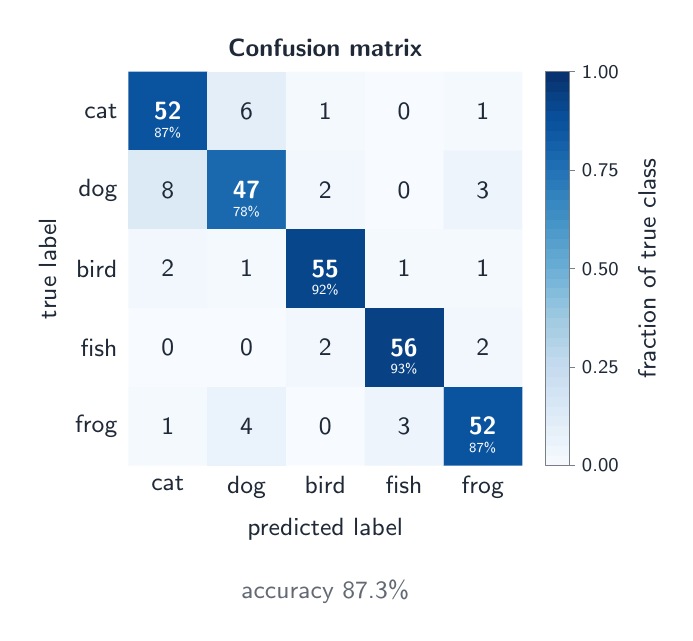
\begin{tikzpicture}[color=Ink, execute at begin picture={\sffamily}, line width=0.6pt, >={Stealth[length=5.5pt, width=4pt, inset=1.2pt]}, line join=round]
  % heatmap hm1 5x5
  \fill[c0A539E] (0,-1) rectangle (1.003,0.003) (4,-5) rectangle (5.003,-3.997);
  \fill[cE3EEF8] (1,-1) rectangle (2.003,0.003);
  \fill[cF4F9FE] (2,-1) rectangle (3.003,0.003) (4,-1) rectangle (5.003,0.003) (1,-3) rectangle
      (2.003,-1.997) (3,-3) rectangle (4.003,-1.997) (4,-3) rectangle (5.003,-1.997) (0,-5) rectangle
      (1.003,-3.997);
  \fill[cF7FBFF] (3,-1) rectangle (4.003,0.003) (3,-2) rectangle (4.003,-0.997) (0,-4) rectangle
      (1.003,-2.997) (1,-4) rectangle (2.003,-2.997) (2,-5) rectangle (3.003,-3.997);
  \fill[cDCEAF6] (0,-2) rectangle (1.003,-0.997);
  \fill[c1A68AE] (1,-2) rectangle (2.003,-0.997);
  \fill[cF1F7FD] (2,-2) rectangle (3.003,-0.997) (0,-3) rectangle (1.003,-1.997) (2,-4) rectangle
      (3.003,-2.997) (4,-4) rectangle (5.003,-2.997);
  \fill[cEDF4FC] (4,-2) rectangle (5.003,-0.997) (3,-5) rectangle (4.003,-3.997);
  \fill[c08468B] (2,-3) rectangle (3.003,-1.997);
  \fill[c084285] (3,-4) rectangle (4.003,-2.997);
  \fill[cEAF2FB] (1,-5) rectangle (2.003,-3.997);
  \node[anchor=east, font=\small, align=center, inner sep=2pt] (hm1-r0) at (-0.06,-0.5) {cat};
  \node[anchor=east, font=\small, align=center, inner sep=2pt] (hm1-r1) at (-0.06,-1.5) {dog};
  \node[anchor=east, font=\small, align=center, inner sep=2pt] (hm1-r2) at (-0.06,-2.5) {bird};
  \node[anchor=east, font=\small, align=center, inner sep=2pt] (hm1-r3) at (-0.06,-3.5) {fish};
  \node[anchor=east, font=\small, align=center, inner sep=2pt] (hm1-r4) at (-0.06,-4.5) {frog};
  \node[anchor=north, font=\small, align=center, inner sep=2pt] (hm1-c0) at (0.5,-5.06) {cat};
  \node[anchor=north, font=\small, align=center, inner sep=2pt] (hm1-c1) at (1.5,-5.06) {dog};
  \node[anchor=north, font=\small, align=center, inner sep=2pt] (hm1-c2) at (2.5,-5.06) {bird};
  \node[anchor=north, font=\small, align=center, inner sep=2pt] (hm1-c3) at (3.5,-5.06) {fish};
  \node[anchor=north, font=\small, align=center, inner sep=2pt] (hm1-c4) at (4.5,-5.06) {frog};
  \node[fit=(hm1-c0)(hm1-c1)(hm1-c2)(hm1-c3)(hm1-c4), inner sep=0pt] (hm1-cols) {};
  \node[anchor=north, font=\small, inner sep=4pt, align=center] at (2.5,0 |- hm1-cols.south) {predicted label};
  \node[fit=(hm1-r0)(hm1-r1)(hm1-r2)(hm1-r3)(hm1-r4), inner sep=0pt] (hm1-rows) {};
  \node[anchor=south, rotate=90, font=\small, inner sep=4pt, align=center] at (hm1-rows.west |- 0,-2.5) {true label};
  \node[anchor=south, font=\small\bfseries, inner sep=4pt, align=center] at (2.5,0.05) {Confusion matrix};
  \fill[cF5F9FE] (5.3,-5) rectangle (5.6,-4.872);
  \fill[cEFF6FC] (5.3,-4.875) rectangle (5.6,-4.747);
  \fill[cEAF3FB] (5.3,-4.75) rectangle (5.6,-4.622);
  \fill[cE6F0F9] (5.3,-4.625) rectangle (5.6,-4.497);
  \fill[cE0ECF8] (5.3,-4.5) rectangle (5.6,-4.372);
  \fill[cDCE9F6] (5.3,-4.375) rectangle (5.6,-4.247);
  \fill[cD7E6F5] (5.3,-4.25) rectangle (5.6,-4.122);
  \fill[cD2E3F3] (5.3,-4.125) rectangle (5.6,-3.997);
  \fill[cCDE0F1] (5.3,-4) rectangle (5.6,-3.872);
  \fill[cC8DCF0] (5.3,-3.875) rectangle (5.6,-3.747);
  \fill[cC2D9EE] (5.3,-3.75) rectangle (5.6,-3.622);
  \fill[cBAD6EB] (5.3,-3.625) rectangle (5.6,-3.497);
  \fill[cB2D2E8] (5.3,-3.5) rectangle (5.6,-3.372);
  \fill[cAACFE5] (5.3,-3.375) rectangle (5.6,-3.247);
  \fill[cA3CCE3] (5.3,-3.25) rectangle (5.6,-3.122);
  \fill[c99C7E0] (5.3,-3.125) rectangle (5.6,-2.997);
  \fill[c8FC2DE] (5.3,-3) rectangle (5.6,-2.872);
  \fill[c84BCDB] (5.3,-2.875) rectangle (5.6,-2.747);
  \fill[c7AB6D9] (5.3,-2.75) rectangle (5.6,-2.622);
  \fill[c71B1D7] (5.3,-2.625) rectangle (5.6,-2.497);
  \fill[c66ABD4] (5.3,-2.5) rectangle (5.6,-2.372);
  \fill[c5FA6D1] (5.3,-2.375) rectangle (5.6,-2.247);
  \fill[c57A0CE] (5.3,-2.25) rectangle (5.6,-2.122);
  \fill[c4E9ACB] (5.3,-2.125) rectangle (5.6,-1.997);
  \fill[c4695C8] (5.3,-2) rectangle (5.6,-1.872);
  \fill[c3E8EC4] (5.3,-1.875) rectangle (5.6,-1.747);
  \fill[c3888C1] (5.3,-1.75) rectangle (5.6,-1.622);
  \fill[c3282BE] (5.3,-1.625) rectangle (5.6,-1.497);
  \fill[c2B7BBA] (5.3,-1.5) rectangle (5.6,-1.372);
  \fill[c2474B7] (5.3,-1.375) rectangle (5.6,-1.247);
  \fill[c1F6EB3] (5.3,-1.25) rectangle (5.6,-1.122);
  \fill[c1967AD] (5.3,-1.125) rectangle (5.6,-0.997);
  \fill[c1561A9] (5.3,-1) rectangle (5.6,-0.872);
  \fill[c0F5AA3] (5.3,-0.875) rectangle (5.6,-0.747);
  \fill[c0A549E] (5.3,-0.75) rectangle (5.6,-0.622);
  \fill[c084E98] (5.3,-0.625) rectangle (5.6,-0.497);
  \fill[c08478D] (5.3,-0.5) rectangle (5.6,-0.372);
  \fill[c084184] (5.3,-0.375) rectangle (5.6,-0.247);
  \fill[c083A7A] (5.3,-0.25) rectangle (5.6,-0.122);
  \fill[c083370] (5.3,-0.125) rectangle (5.6,0);
  \draw[Ink!60, line width=0.4pt] (5.3,-5) rectangle (5.6,0);
  \draw[Ink!60, line width=0.4pt] (5.6,-5) -- (5.67,-5);
  \node[anchor=west, font=\scriptsize, inner sep=2pt] at (5.68,-5) {0.00};
  \draw[Ink!60, line width=0.4pt] (5.6,-3.75) -- (5.67,-3.75);
  \node[anchor=west, font=\scriptsize, inner sep=2pt] at (5.68,-3.75) {0.25};
  \draw[Ink!60, line width=0.4pt] (5.6,-2.5) -- (5.67,-2.5);
  \node[anchor=west, font=\scriptsize, inner sep=2pt] at (5.68,-2.5) {0.50};
  \draw[Ink!60, line width=0.4pt] (5.6,-1.25) -- (5.67,-1.25);
  \node[anchor=west, font=\scriptsize, inner sep=2pt] at (5.68,-1.25) {0.75};
  \draw[Ink!60, line width=0.4pt] (5.6,0) -- (5.67,0);
  \node[anchor=west, font=\scriptsize, inner sep=2pt] at (5.68,0) {1.00};
  \node[anchor=north, rotate=90, font=\small] at (6.35,-2.5) {fraction of true class};
  \node[font=\small, text=white] at (0.5,-0.5) {\textbf{52}};
  \node[font=\tiny, text=white] at (0.5,-0.77) {87\%};
  \node[font=\small, text=Ink] at (1.5,-0.5) {6};
  \node[font=\small, text=Ink] at (2.5,-0.5) {1};
  \node[font=\small, text=Ink] at (3.5,-0.5) {0};
  \node[font=\small, text=Ink] at (4.5,-0.5) {1};
  \node[font=\small, text=Ink] at (0.5,-1.5) {8};
  \node[font=\small, text=white] at (1.5,-1.5) {\textbf{47}};
  \node[font=\tiny, text=white] at (1.5,-1.77) {78\%};
  \node[font=\small, text=Ink] at (2.5,-1.5) {2};
  \node[font=\small, text=Ink] at (3.5,-1.5) {0};
  \node[font=\small, text=Ink] at (4.5,-1.5) {3};
  \node[font=\small, text=Ink] at (0.5,-2.5) {2};
  \node[font=\small, text=Ink] at (1.5,-2.5) {1};
  \node[font=\small, text=white] at (2.5,-2.5) {\textbf{55}};
  \node[font=\tiny, text=white] at (2.5,-2.77) {92\%};
  \node[font=\small, text=Ink] at (3.5,-2.5) {1};
  \node[font=\small, text=Ink] at (4.5,-2.5) {1};
  \node[font=\small, text=Ink] at (0.5,-3.5) {0};
  \node[font=\small, text=Ink] at (1.5,-3.5) {0};
  \node[font=\small, text=Ink] at (2.5,-3.5) {2};
  \node[font=\small, text=white] at (3.5,-3.5) {\textbf{56}};
  \node[font=\tiny, text=white] at (3.5,-3.77) {93\%};
  \node[font=\small, text=Ink] at (4.5,-3.5) {2};
  \node[font=\small, text=Ink] at (0.5,-4.5) {1};
  \node[font=\small, text=Ink] at (1.5,-4.5) {4};
  \node[font=\small, text=Ink] at (2.5,-4.5) {0};
  \node[font=\small, text=Ink] at (3.5,-4.5) {3};
  \node[font=\small, text=white] at (4.5,-4.5) {\textbf{52}};
  \node[font=\tiny, text=white] at (4.5,-4.77) {87\%};
  \node[font=\small, text=Ink!70] at (2.5,-6.6) {accuracy 87.3\%};
\end{tikzpicture}
\end{document}
